\section{Implementation}

\subsection{Framework}
This pipeline was developed in MATLAB. Since the group consists of four students, a Git repository was used to be able to work on different files simultaneously, and to enable version control.
(keywords: MATLAB, Git)

\subsubsection{Coordinate Frames}
In this mini project the coordinate frames were defined as shown in \cref{img_coord_frames}. The camera coordinates are in a way oriented, that the x-y plane lies parallel to the image plane, while the z-axis is pointing towards the scenery. The world frame however is oriented in such a way that the x-y plane is parallel to the ground and the the z-axis is pointing upwards.

The origin of the world frame is at the same location as the origin of the first boot-strap image.

\begin{figure}[ht]
	\centering
	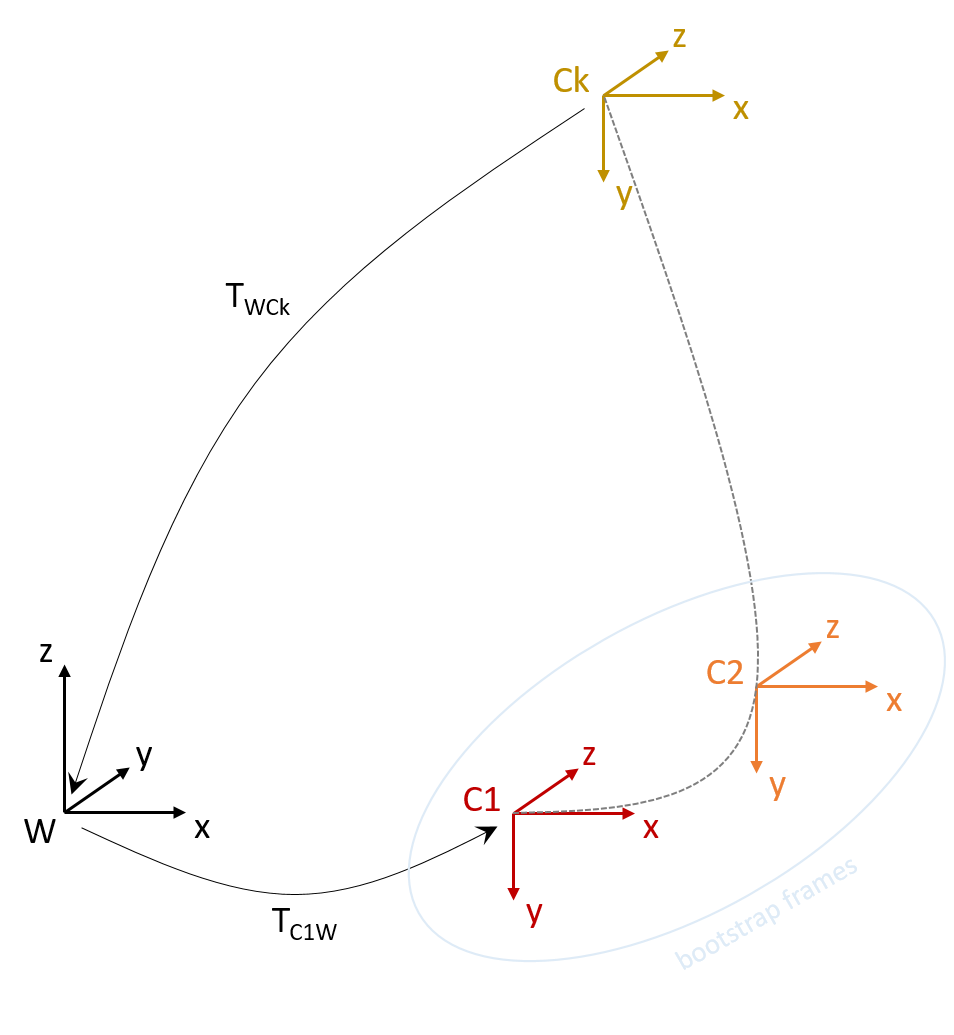
\includegraphics[width=0.5\textwidth]{coord_frames}
	\caption{Coordinate Frames}
	\label{img_coord_frames}
\end{figure}

\subsubsection{Pipeline overview}

As shown in \cref{img_flow_rough} the pipeline consists mainly of three parts, a bootstrap, the initialisation and the continuous operation. In \cref{sec_init} and \cref{sec_cont_op} the initialisation and the continuous operation are described in detail.

\begin{figure}[ht]
	\centering
	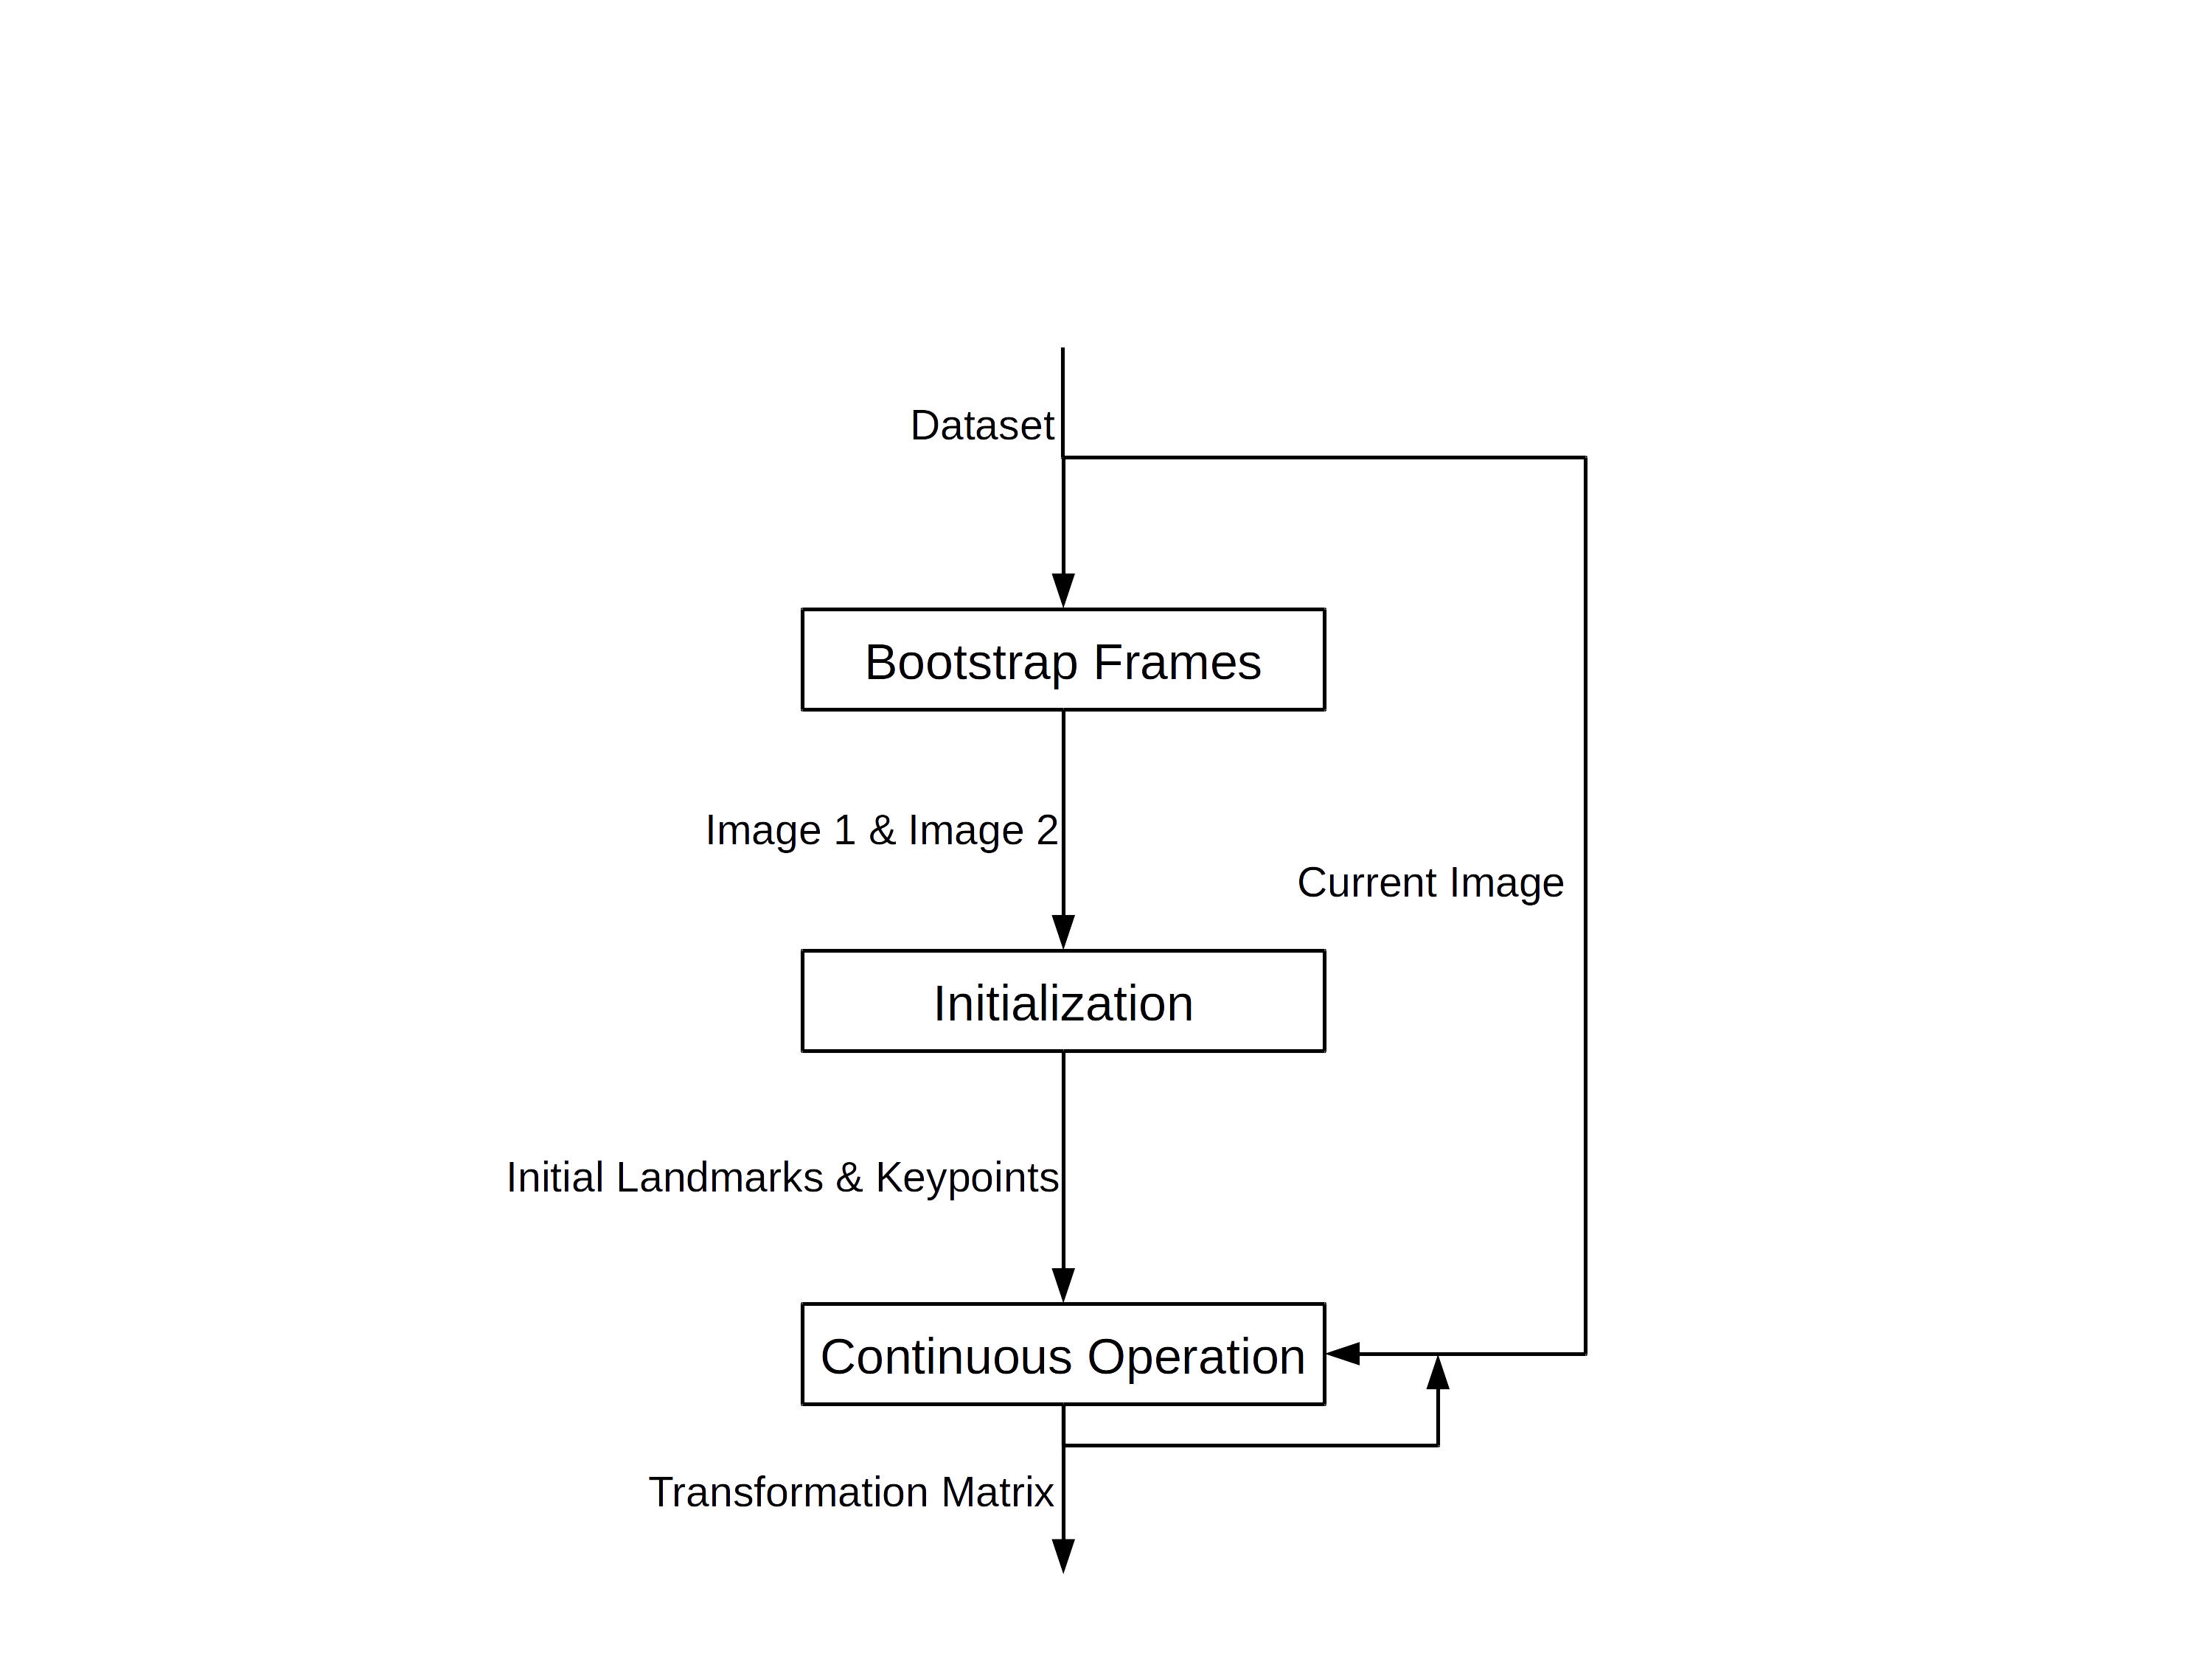
\includegraphics[width=0.8\textwidth]{rough_flow}
	\caption{Rough Flow chart}
	\label{img_flow_rough}
\end{figure}
%\input{pipeline_overview}
\subsubsection{Options and parameters}
(keywords: parameter handling, GUI)


\subsection{Initialization}
\label{sec_init}


\begin{figure}[ht]
	\centering
	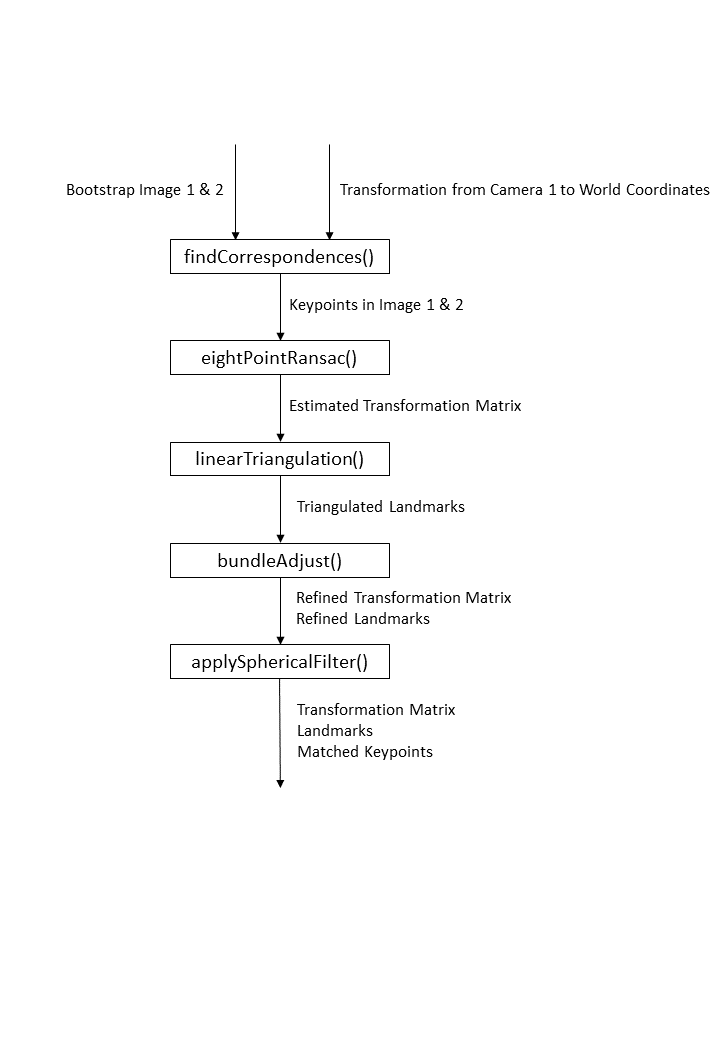
\includegraphics[width=0.8\textwidth]{init_chart}
	\caption{Init Flow chart}
	\label{img_flow_init}
\end{figure}
\clearpage{\pagestyle{plain}\cleardoublepage}
\subsection{Continuous Operation}
\label{sec_cont_op}


\begin{figure}[ht]
	\centering
	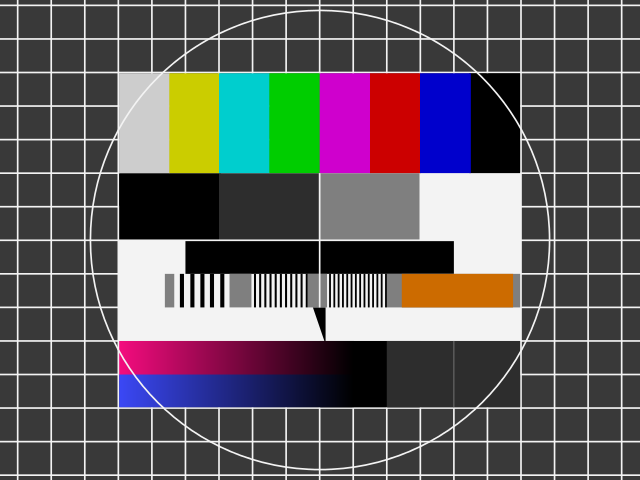
\includegraphics[width=0.8\textwidth]{test}
	\caption{Cont Flow chart}
	\label{img_flow_cont}
\end{figure}
\clearpage{\pagestyle{plain}\cleardoublepage}